\documentclass[10pt,a4paper]{article}

\usepackage[T1]{fontenc}
\usepackage[utf8]{inputenc}
\usepackage[margin=2cm]{geometry}
\usepackage{amsmath,amssymb}
\usepackage{graphicx}
\usepackage{booktabs}
\usepackage{microtype}
\usepackage[font=small,labelfont=bf,skip=6pt]{caption}
\usepackage[colorlinks=true,linkcolor=black,citecolor=black,urlcolor=blue]{hyperref}

\graphicspath{{../figures/}}
\setlength{\parskip}{0.55em}
\setlength{\parindent}{0pt}
\linespread{1.02}

\title{\vspace{-1.4cm}\textbf{Face Recognition Using Eigenfaces\\and Pattern Classification}}
\author{Daniel Kpakpo Adotey~~\textbar~~ID 22424924\\
\texttt{dkadotey@st.ug.edu.gh}\\[0.35em]
DSCD612 Pattern Recognition, Project 3\\
MPhil/MSc Data Science, University of Ghana}
\date{Second Semester, 2025/2026}

\begin{document}
\maketitle
\vspace{-0.7cm}

%======================================================================
\section{Problem and dataset}
%======================================================================

Closed-set face identification asks which of $C$ enrolled individuals a given
image depicts. Posed directly in pixel space the problem is badly conditioned:
a $64\times64$ greyscale image is a point in $\mathbb{R}^{4096}$ and the dataset
used here supplies 400 such points, so features outnumber observations by about
ten to one. The sample covariance matrix is singular by construction and no
per-class density is estimable.

Face images do not fill $\mathbb{R}^{4096}$. They concentrate near a much
lower-dimensional structure, because faces share a common geometry. The
Eigenfaces method \cite{turk1991} exploits this: it finds the linear subspace
holding most of the variation across a set of faces, then recognises inside it.
This report implements that pipeline from first principles, including the
principal component analysis itself, to answer the project's central question:

\begin{quote}
How much dimensionality can be removed from facial images before
identity-discriminating information is significantly lost?
\end{quote}

The question admits two different measurements. \emph{Reconstruction} asks how
much pixel variance survives; \emph{discrimination} asks how well identities can
still be told apart. The main finding here is that the two criteria disagree by
a factor of about four, for a reason that the component structure explains.

The \textbf{Olivetti (ORL) database} \cite{samaria1994} supplies 400 greyscale
images of 40 subjects, ten each, normalised to $[0,1]$. Within a subject the
images vary in lighting, expression, and the presence of glasses. All are
cropped, frontal, and roughly aligned against a dark background, so this study
measures the recognition method rather than a face \emph{detection} front end.
The redundancy that motivates the method is measurable: among 300 sampled pixels
the mean absolute pairwise correlation is $0.26$ and $10.4\%$ of pairs exceed
$|r|=0.5$.

%======================================================================
\section{Method}
%======================================================================

\subsection{Representation and principal component analysis}

Each image is flattened row-major into $x_i\in\mathbb{R}^{d}$, $d=4096$, and
stacked into $X=[x_1,\dots,x_N]^{T}$ with $N=400$. Writing
$\mu=\frac{1}{N}\sum_i x_i$ and $A=X-\mathbf{1}\mu^{T}$, the sample covariance is
\begin{equation}
\Sigma=\frac{1}{N-1}\sum_{i=1}^{N}(x_i-\mu)(x_i-\mu)^{T}=\frac{1}{N-1}A^{T}A.
\label{eq:cov}
\end{equation}

PCA maximises the projected variance $v^{T}\Sigma v$ subject to $v^{T}v=1$. With
a Lagrange multiplier, $\mathcal{L}=v^{T}\Sigma v-\lambda(v^{T}v-1)$, and
$\partial\mathcal{L}/\partial v=0$ yields the eigenvalue problem
\begin{equation}
\Sigma v_i=\lambda_i v_i .
\label{eq:eig}
\end{equation}

The stationary points of the projected variance are the eigenvectors of
$\Sigma$, and since $v_i^{T}\Sigma v_i=\lambda_i$, each eigenvalue is the
variance along its own direction. Keeping the top $k$ eigenvectors as columns of
$W_k$ gives the rank-$k$ subspace of least expected squared reconstruction error
(Eckart--Young \cite{eckart1936}). $\Sigma$ is real symmetric, so
$W_k^{T}W_k=I_k$.

\subsection{The snapshot trick}

$\Sigma$ is $4096\times4096$ and singular: it sums $N_{\text{train}}$ rank-one
terms under one linear constraint, so
$\operatorname{rank}(\Sigma)\le N_{\text{train}}-1=279$ and at most 279 of its
4096 eigenvalues are non-zero. Take instead the Gram matrix
$G=\frac{1}{N-1}AA^{T}\in\mathbb{R}^{N\times N}$. If $Gu_i=\lambda_i u_i$,
left-multiplying by $A^{T}$ gives
\begin{equation}
\frac{1}{N-1}A^{T}AA^{T}u_i=\lambda_i A^{T}u_i
\iff \Sigma\,(A^{T}u_i)=\lambda_i\,(A^{T}u_i),
\label{eq:snapshot}
\end{equation}
so $A^{T}u_i$ is an eigenvector of $\Sigma$ carrying the same eigenvalue. The
non-zero spectrum of a $4096\times4096$ matrix therefore follows from an
$N\times N$ eigenproblem, $280\times280$ when fitting on a training split, and
the cost of the decomposition falls from $O(d^{3})$ to $O(N^{3})$. Benchmarked
on the full 400-image matrix this is a reduction of roughly two orders of
magnitude. The exact ratio depends on the hardware and on the BLAS
implementation, so the notebook measures it on each run rather than fixing a
figure here. The resulting vectors are normalised to unit length.

Each $v_i$ lies in $\mathbb{R}^{4096}$, the space of the images themselves, so
it reshapes to $64\times64$ and displays as a \emph{pattern of deviation from
the mean face}. Being a linear combination of training faces,
$v_i\propto\sum_j u_{ij}(x_j-\mu)$, it inherits their face-like structure, hence
the name, and any face is then a recipe of $k$ coefficients over that shared
basis: $x\approx\mu+\sum_{j\le k} z_jv_j$ with $z=W_k^{T}(x-\mu)$.

\subsection{Classification and verification}

A test face is projected to $z=W_k^{T}(x-\mu)$ and classified by $k$-nearest
neighbours \cite{duda2001}. The non-parametric rule is a necessity here rather
than a preference. With 40 classes and 7 training images each, a full Gaussian
per class would need $k+k(k+1)/2$ parameters from 7 observations. Because $W_k$
is orthonormal, distances in the projected space equal distances between the
pixel-space reconstructions. Two variants recur: \textbf{plain} projection,
where components keep their natural scale so high-variance directions dominate,
and \textbf{whitened} projection $\tilde z_j=z_j/\sqrt{\lambda_j}$, which
rescales every component to unit variance and amounts to a Mahalanobis distance
inside the retained subspace.

Checked against scikit-learn's exact SVD solver, the implementation gives a
maximum relative eigenvalue error of $5.0\times10^{-15}$, a minimum absolute
eigenvector dot product of $1.0000000000$, and a maximum reconstruction
difference of $1.6\times10^{-14}$.

%======================================================================
\section{Experimental design}
%======================================================================

Each subject contributes $n_{\text{train}}$ images to training and the rest to
test, since a uniformly random split would leave some subjects with no training
images and so unidentifiable by construction. The default is 7 train / 3 test
per subject: $N_{\text{train}}=280$, $N_{\text{test}}=120$.

$\mu$ and $W$ come from training images only, and test images are projected
using those fixed parameters, because fitting PCA on all 400 images before
splitting leaks information into the basis and inflates the accuracy reported
from it. With 120 test images a single split carries a standard error near 2.4
percentage points, so every figure reported here averages \textbf{10}
independent splits and carries its standard deviation.

One caveat applies to the choice of $k$ and is stated here rather than left
implicit. Two values recur below: $k=75$, the position of the maximum of the
mean accuracy curve, and $k=25$, the smallest $k$ whose mean accuracy lies
within one standard deviation of that maximum. Both were read off the same
test splits that the results are reported on, so neither is a clean held-out
estimate, and the figures quoted at those $k$ carry some optimism. The
accuracy curve bounds it: plain projection moves from $0.926$ at $k=25$ to
$0.937$ at its peak and stays flat to $k=279$, a span of about one point,
which is within the split-to-split standard deviation of $0.013$. Selecting
$k$ on a validation partition carved out of the training images would remove
the dependence altogether, and is the correct construction where the choice of
$k$ has to carry more weight than it does here.

%======================================================================
\section{Results}
%======================================================================

\begin{figure}[htbp]
\centering
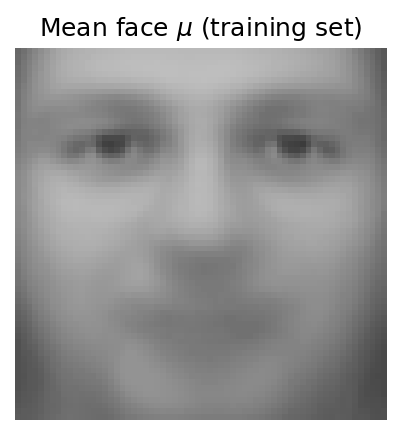
\includegraphics[width=0.24\textwidth]{05_mean_face_train.png}
\caption{The mean face $\mu$, averaged over the 280 training images. Every
Eigenface below is a pattern of deviation from this image, and every
reconstruction begins here.}
\label{fig:meanface}
\end{figure}

Figure~\ref{fig:meanface} shows $\mu$. It is a blurred, generic frontal face,
which is what the average of 40 identities under varying expression and
lighting should look like: the features that all faces share survive the
averaging and everything identifying cancels. Subtracting it is what makes the
first component describe variation between faces rather than the shared
structure common to all of them.

\begin{figure}[htbp]
\centering
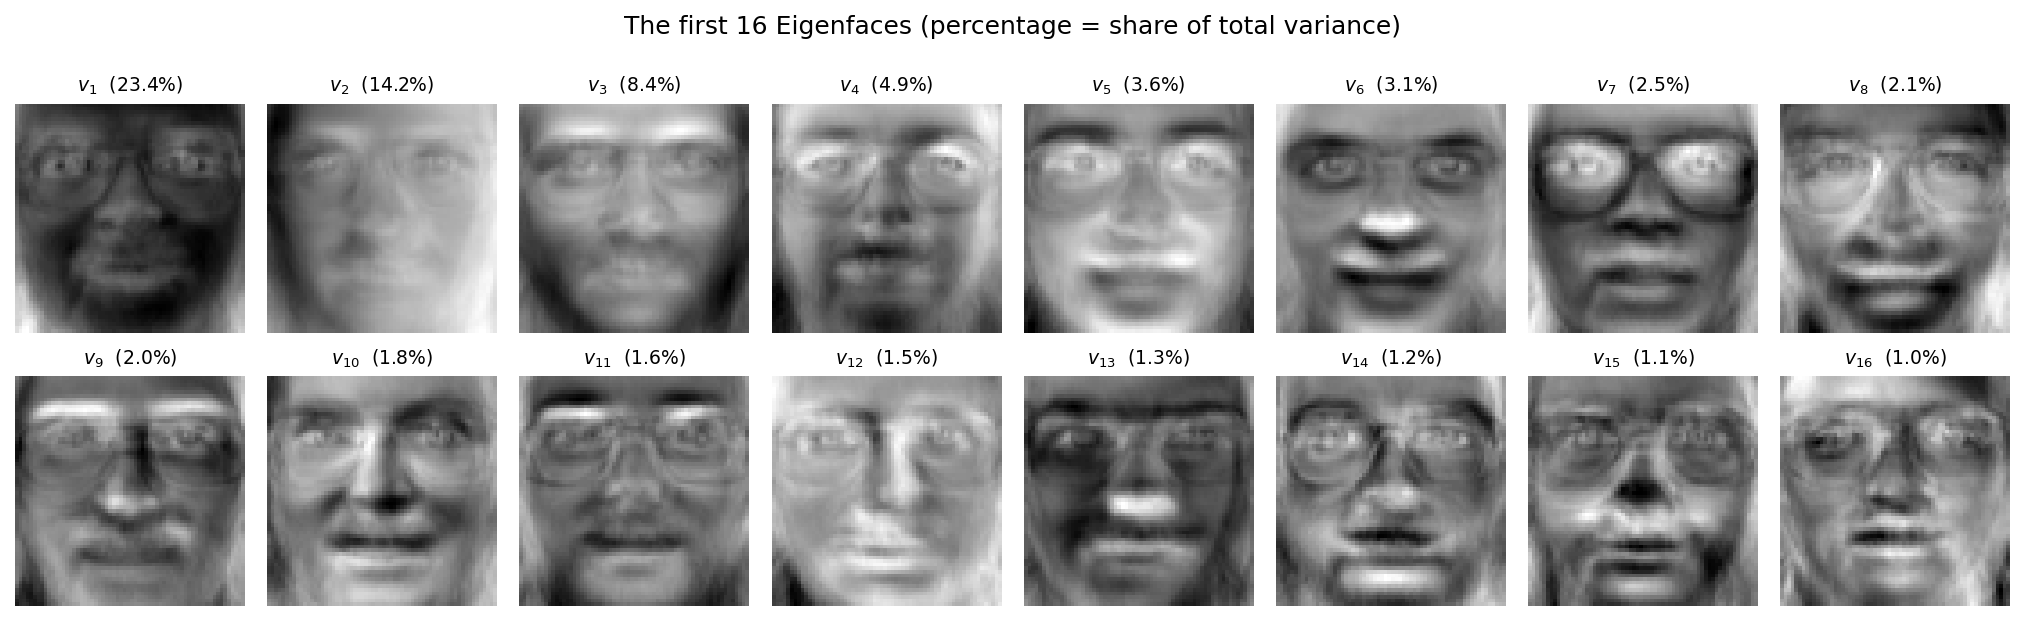
\includegraphics[width=0.94\textwidth]{06_eigenfaces.png}
\caption{The first 16 Eigenfaces, with each component's share of total variance.}
\label{fig:eigenfaces}
\end{figure}

The first three components in Figure~\ref{fig:eigenfaces} are low in spatial
frequency and describe whole-image photometric structure rather than facial
detail. $v_1$ is a broad contrast pattern separating the brow and eye band from
the rest of the face, $v_2$ is nearly flat and encodes overall luminance, and
$v_3$ carries a top-to-bottom intensity gradient. None of them describes who the
person is. Recognisable structure begins at $v_4$: spectacle frames,
hairline, moustaches, and changes around the mouth. Later components grow more
localised and higher in frequency, carrying identity information alongside
sampling noise specific to these training images.

The conventional variance thresholds need 59, 103, and 198 components
for 90\%, 95\%, and 99\% respectively, that is 1.44\%, 2.51\%, and 4.83\% of the
original 4096 dimensions. The first component alone holds 23.4\% of total
variance and the first ten hold 66.1\%.

\begin{figure}[htbp]
\centering
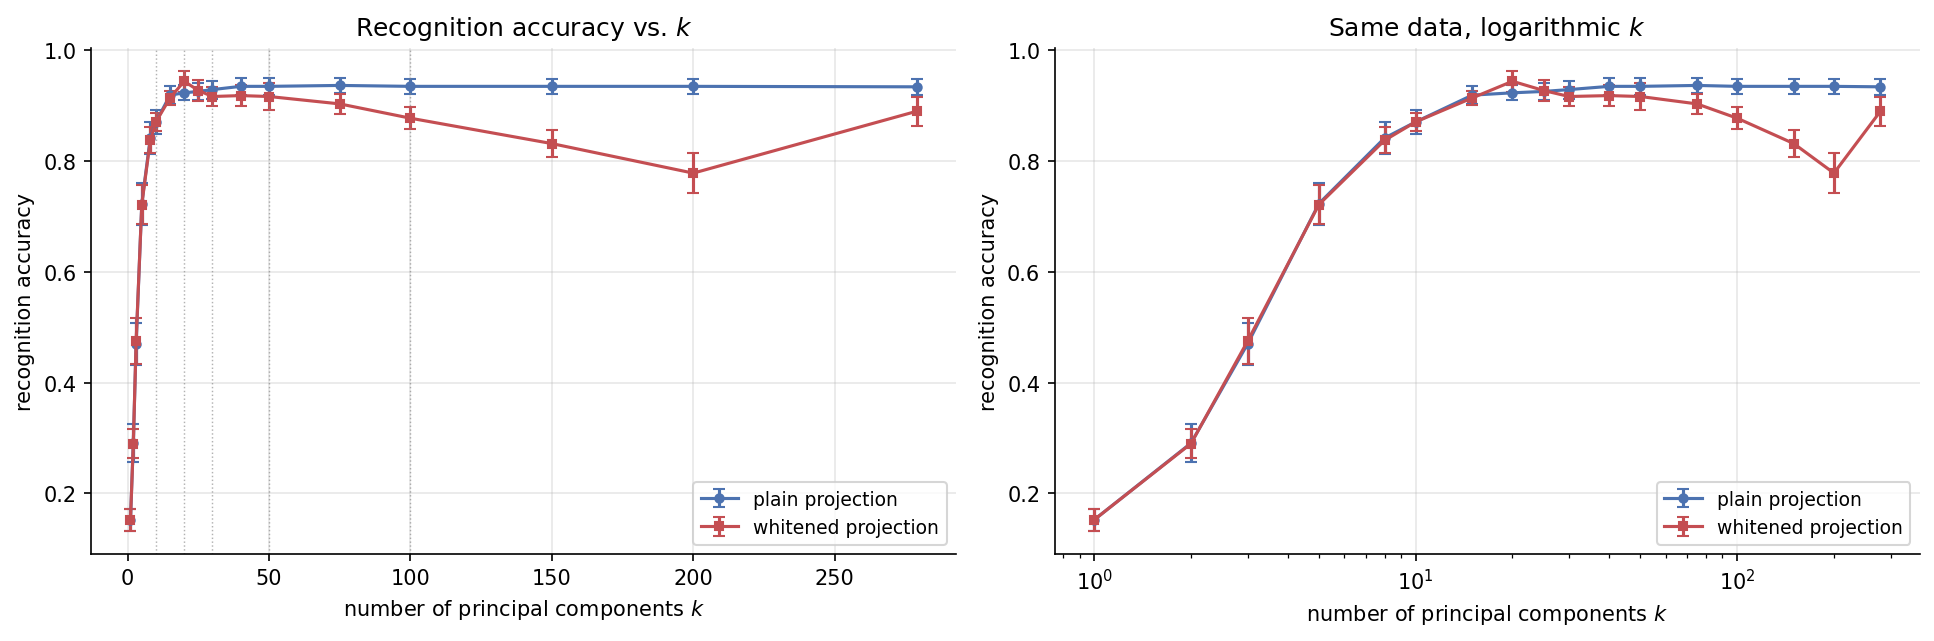
\includegraphics[width=0.72\textwidth]{08_accuracy_vs_k.png}
\caption{Recognition accuracy against $k$, plain and whitened projections,
mean $\pm$ s.d.\ over 10 splits.}
\label{fig:acc}
\end{figure}

\begin{table}[htbp]
\centering
\caption{Recognition accuracy against the number of retained components.}
\label{tab:acc}
\begin{tabular}{rll@{\hskip 2.2em}rll}
\toprule
$k$ & Plain & Whitened & $k$ & Plain & Whitened\\
\midrule
10 & $0.871\pm0.021$ & $0.871\pm0.017$ & 50  & $0.935\pm0.015$ & $0.917\pm0.025$\\
20 & $0.923\pm0.014$ & $\mathbf{0.944}\pm0.019$ & 75  & $\mathbf{0.937}\pm0.013$ & $0.903\pm0.018$\\
25 & $0.926\pm0.016$ & $0.928\pm0.020$ & 100 & $0.935\pm0.013$ & $0.878\pm0.020$\\
30 & $0.929\pm0.016$ & $0.917\pm0.017$ & 200 & $0.935\pm0.013$ & $0.778\pm0.036$\\
\bottomrule
\end{tabular}
\end{table}

The two curves in Figure~\ref{fig:acc} behave differently, and the contrast
between them is the clearest result here.

The plain curve rises and then flattens rather than falling, which follows from
the geometry rather than from the dataset. $W$ is orthonormal, so with every
component retained the Euclidean distance in Eigenface space equals the pixel
distance exactly, and adding components moves 1-NN monotonically towards the
full-dimensional answer. Trailing components carry tiny eigenvalues and
contribute almost nothing to a Euclidean distance, so under this metric keeping
too many components costs computation rather than accuracy.

The whitened curve rises, peaks at $k=20$, then falls from $0.944$ to $0.778$ at
$k=200$. Whitening divides component $j$ by $\sqrt{\lambda_j}$, which for a
trailing component means dividing by a very small number and so promoting it to
equal footing with the leading ones. The $i$-th eigenvalue, however, comes from
280 observations in 4096 dimensions. For large $i$ that estimate is dominated by
sampling noise, and the direction then describes quirks of the particular
training images rather than a property of the population. Whitening amplifies
exactly that noise, producing the familiar overfitting signature.

Both curves point at one principle. The useful number of components is set by
how many directions the sample estimates reliably, not by how many exist
mathematically, and whether the unreliable ones do damage depends on whether the
metric gives them weight. That is why the curves diverge, and why ``how many
components should I keep?'' has no answer the representation alone can supply.

At $k=75$, 1-NN with Euclidean distance gives accuracy $0.9367\pm0.0137$, macro
precision $0.9507$, macro recall $0.9367$, and macro $F_1$ $0.9339$.
Macro-averaging weights every subject equally, so failure on a few individuals
cannot hide behind a good average. On the reference split 8 of 120 test images
are misclassified and the confusion matrix is almost entirely diagonal, with no
pair of subjects mutually confused.

Across distances at $k=75$, Manhattan reaches $0.9442$ against Euclidean's
$0.9367$ and cosine's $0.9300$ at 1-NN, a margin well under one standard
deviation. The dominant effect is neighbourhood size rather than the distance
function. Euclidean accuracy falls to $0.854$ at 3-NN and $0.805$ at 5-NN. With
7 training images per subject a 5-NN vote often reaches past the correct
identity into neighbouring clusters, so the usual argument that larger $n$
smooths noise assumes a sample density this problem lacks.

\subsection{Reconstruction}

\begin{figure}[htbp]
\centering
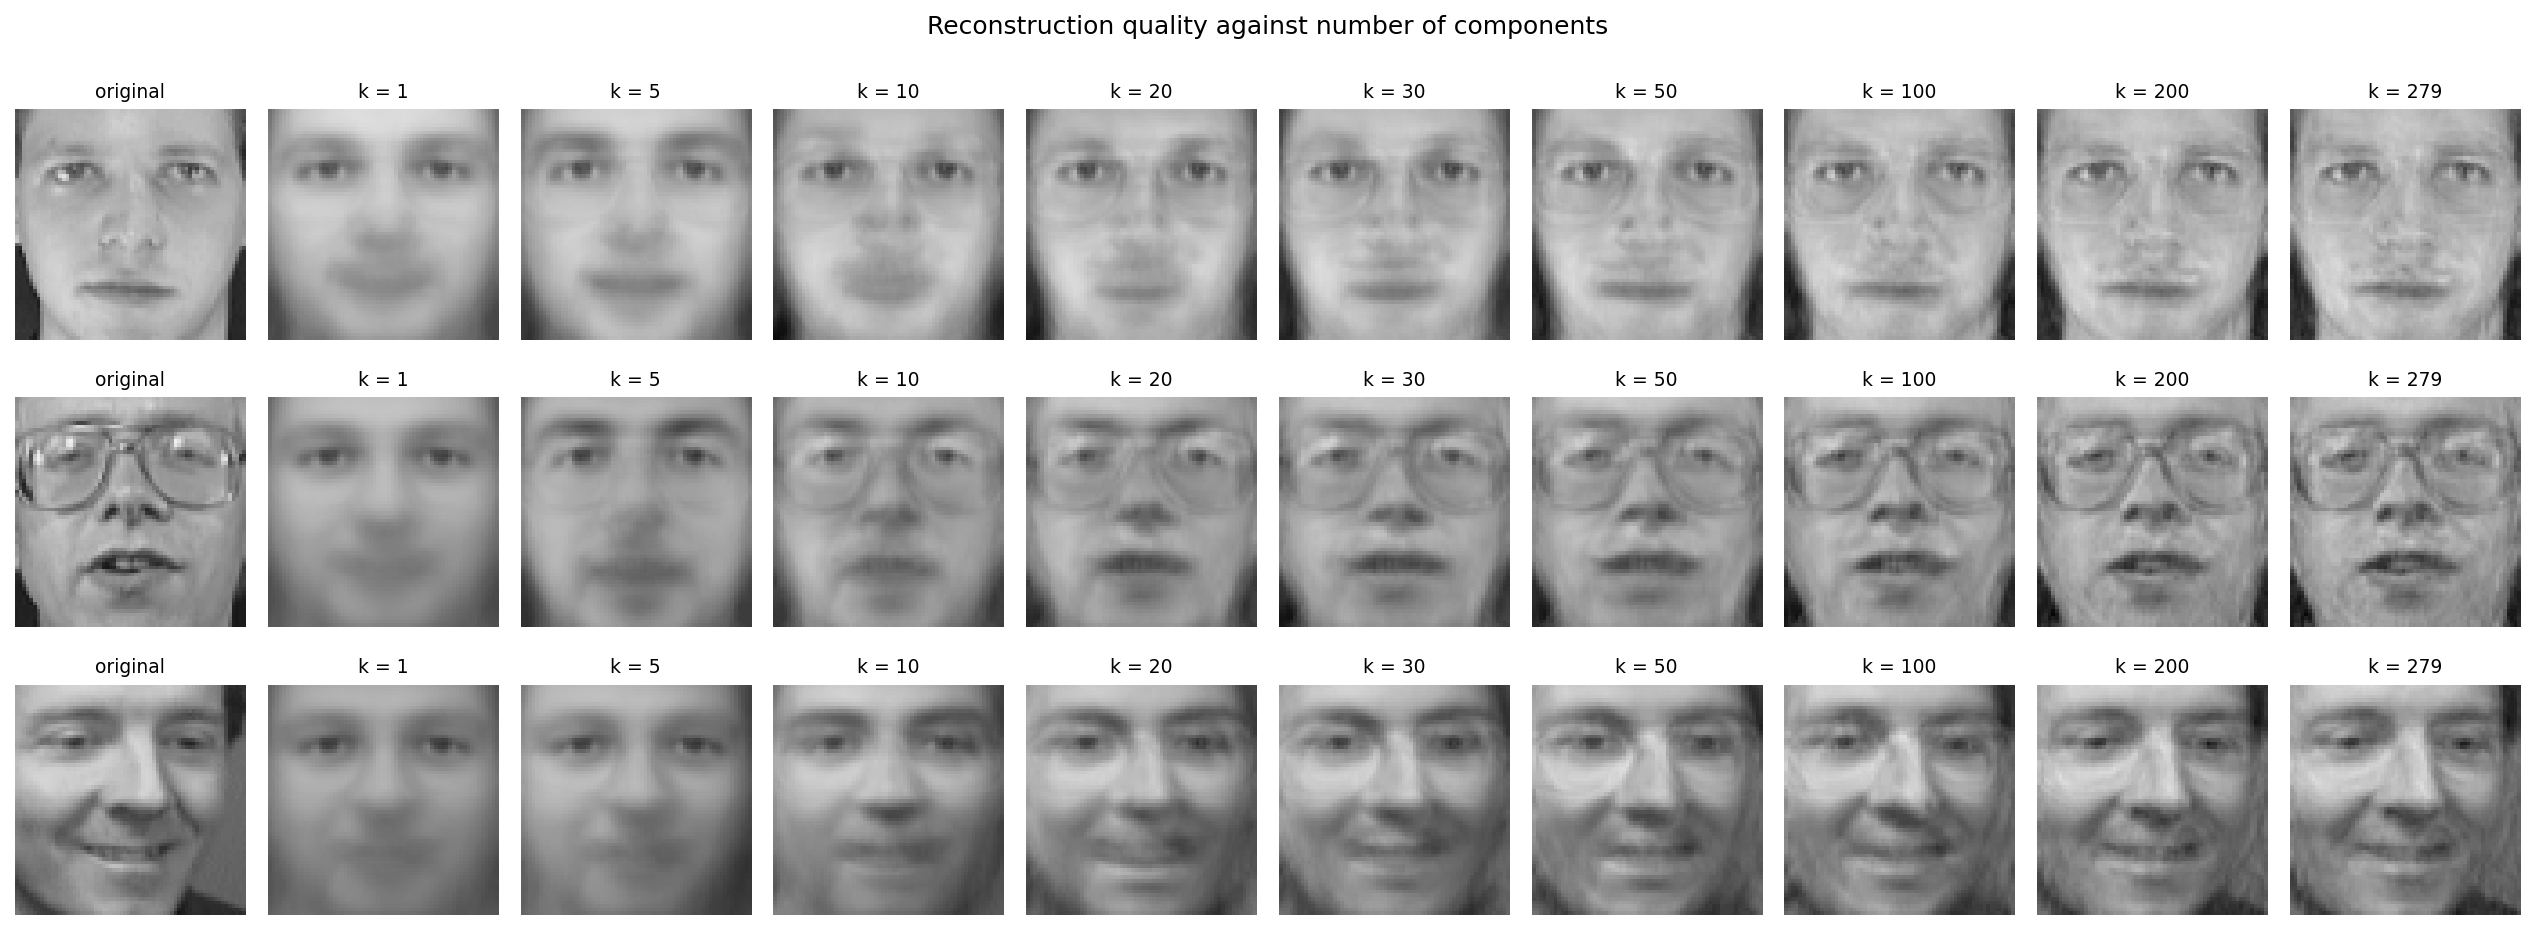
\includegraphics[width=0.80\textwidth]{12_reconstructions.png}
\caption{Reconstructions of three test faces at increasing $k$.}
\label{fig:recon}
\end{figure}

Reconstruction maps a projection back by $\hat x=\mu+W_kW_k^{T}(x-\mu)$, and
since $W_kW_k^{T}$ is an orthogonal projector, the residual lies wholly in the
discarded directions, giving
$\mathbb{E}\|x-\hat x\|^2=\sum_{j>k}\lambda_j$. In Figure~\ref{fig:recon}, at
$k=1$ every face is the mean face with a photometric adjustment. Identity
becomes visually recognisable around $k=20$ to $30$, and past $k\approx100$ the
changes are confined to fine texture. Test RMSE falls from $0.083$ at $k=10$ to
$0.050$ at $k=100$ and $0.041$ at $k=279$, with PSNR $21.8$, $26.2$, and
$28.1$~dB.

\begin{figure}[htbp]
\centering
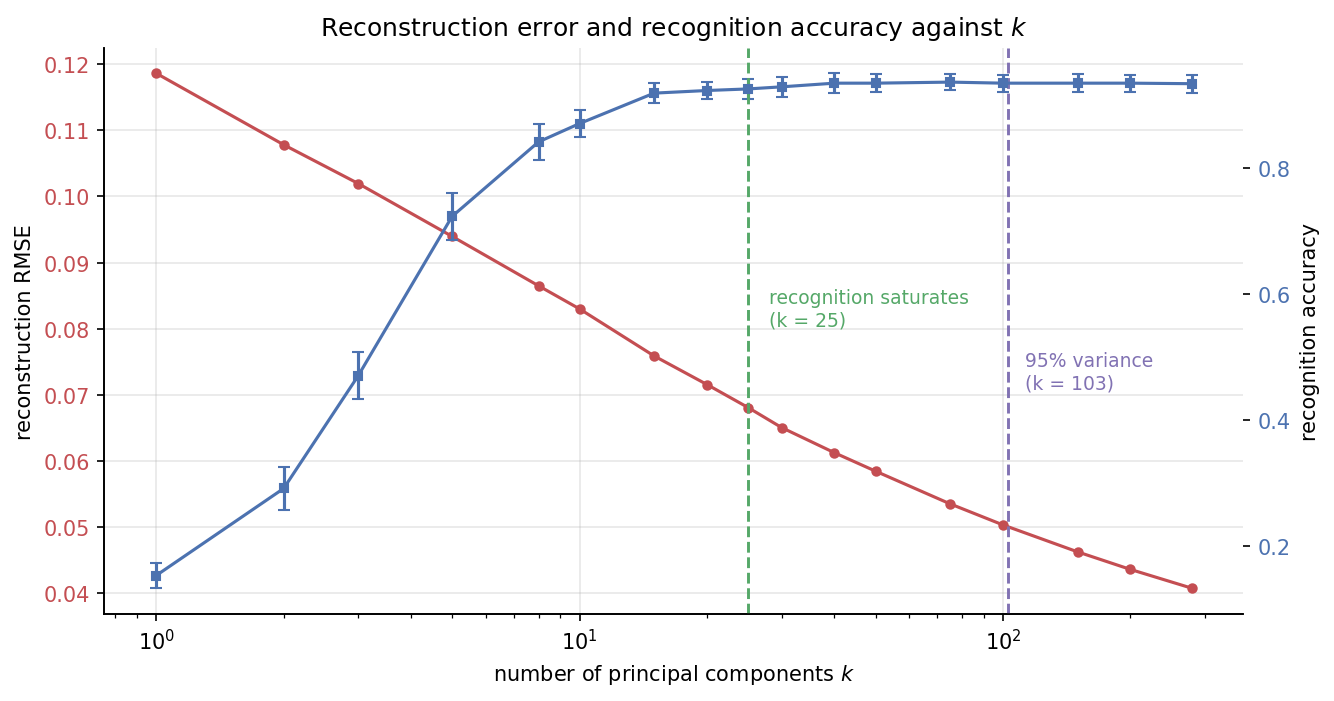
\includegraphics[width=0.62\textwidth]{13_recon_vs_recognition.png}
\caption{Reconstruction error and recognition accuracy against $k$.}
\label{fig:diverge}
\end{figure}

Reconstruction error keeps falling well past the point where recognition stops
improving, because the variance removed across that range, fine skin texture,
sensor noise, small expression detail, feeds pixel fidelity and not identity.
Holding 95\% of variance costs about four times the components recognition
needs, $k=103$ against $k=25$, and buys roughly one accuracy point, which sits
inside the split-to-split noise. A variance threshold is therefore the wrong
criterion for choosing $k$ in a recogniser: it measures how well the subspace
reproduces images, where recognition needs it to separate identities.

%======================================================================
\section{Critical analysis}
%======================================================================

\textbf{Enrolment set size} is the strongest single influence measured. Accuracy
runs $0.547$, $0.698$, $0.774$, $0.820$, $0.867$, $0.923$, and $0.950$ for 1, 2,
3, 4, 5, 7, and 9 training images per subject, and has not saturated at nine. Two
mechanisms compound. The classifier holds few reference points, so a test image
with an unseen expression has no near neighbour of the correct identity; and the
basis itself degrades, since at $n_{\text{tr}}=1$ only 39 components exist,
estimated from 40 images. The 40-point drop from nine images to one is the
familiar one-sample-per-person difficulty.

\textbf{Illumination.} Test images were multiplied by a left-to-right linear
intensity ramp of increasing strength, modelling a directional source absent at
enrolment, with training images untouched.

\begin{table}[htbp]
\centering
\caption{Recognition accuracy under increasing illumination mismatch.}
\label{tab:illum}
\begin{tabular}{lcccccc}
\toprule
Ramp strength & 0.0 & 0.2 & 0.3 & 0.4 & 0.5 & 0.7\\
\midrule
Euclidean    & 0.937 & 0.878 & 0.758 & 0.488 & 0.305 & 0.142\\
Cosine       & 0.930 & 0.869 & 0.726 & 0.471 & 0.308 & 0.181\\
Drop first 3 & 0.932 & \textbf{0.938} & \textbf{0.936} & \textbf{0.920} & \textbf{0.890} & \textbf{0.783}\\
\bottomrule
\end{tabular}
\end{table}

\begin{figure}[htbp]
\centering
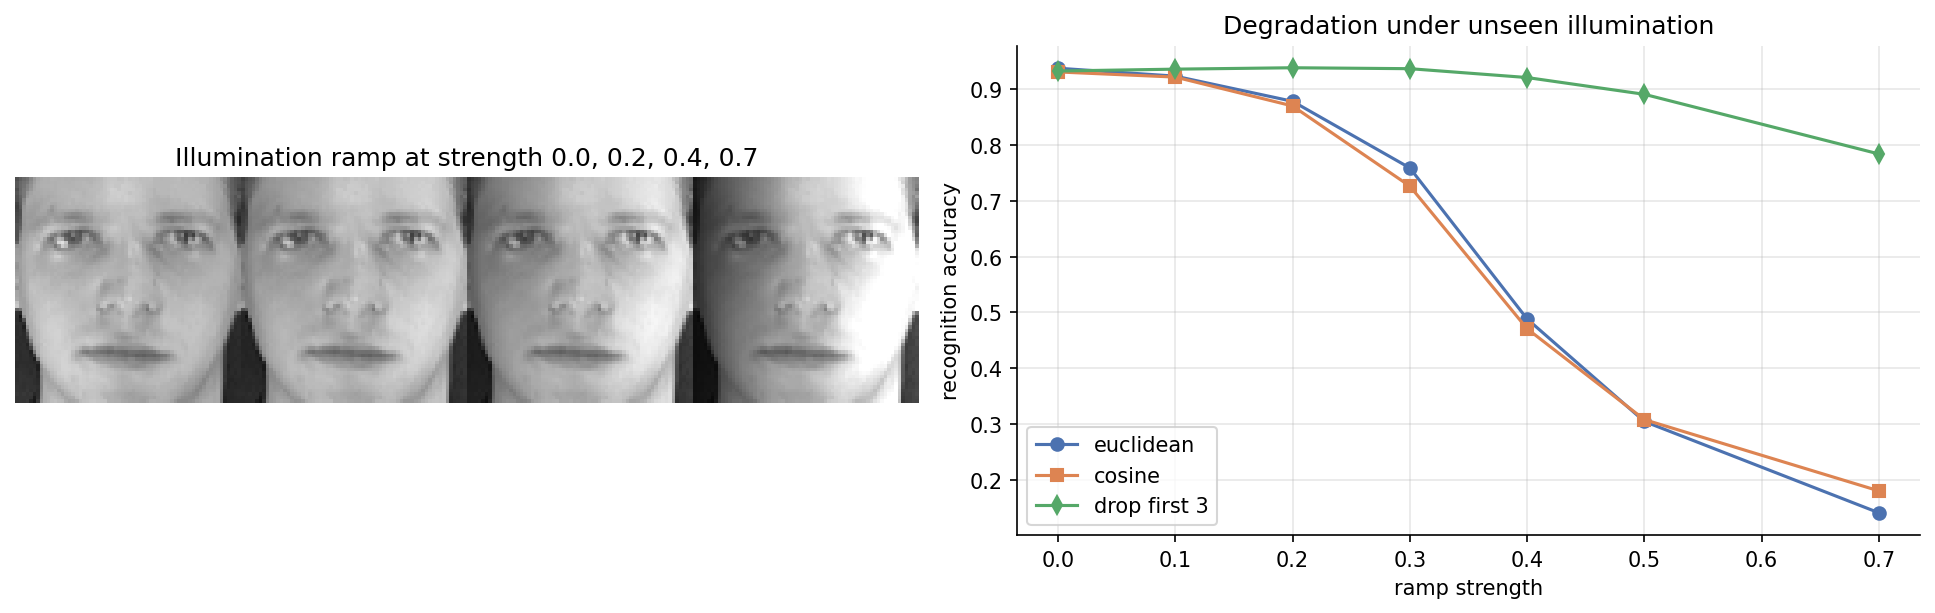
\includegraphics[width=0.76\textwidth]{15_illumination.png}
\caption{Left: the ramp at strengths 0.0, 0.2, 0.4, 0.7. Right: accuracy under
increasing illumination mismatch.}
\label{fig:illum}
\end{figure}

Euclidean 1-NN collapses. Of the two mitigations tested, only one works.

Cosine distance does not help, tracking the Euclidean result at every strength,
because the expectation that it would help assumed a uniform brightness change,
which shifts a projection mainly in magnitude. This ramp varies spatially,
brightening one side of the face and darkening the other, so it rotates the
projection rather than lengthening it, and discarding magnitude discards nothing
relevant. Invariance to global scaling buys little against lighting with spatial
structure, which real lighting always has.

Discarding the first three components does work. At the strongest ramp Euclidean
1-NN falls to $0.142$ while the same classifier without those components holds
$0.783$, so those three directions absorb nearly the whole perturbation. This is
experimental support for the reading of the component structure given earlier:
the leading eigenfaces encode photometric conditions rather than identity.
Discarding the three directions that carry the largest share of variance in the
entire dataset improves recognition under illumination change. At the top of
the spectrum, variance ranking and discriminative value work against each
other.

Under matched illumination, dropping up to three components moves accuracy by
less than one standard deviation either way, and dropping beyond about five
costs real accuracy. Removing three discards 46\% of total variance and leaves
recognition unchanged. Discarding leading components is therefore insurance
against mismatched conditions rather than a free gain.

%======================================================================
\section{Answering the research question}
%======================================================================

1-NN on the raw 4096 pixels, with no reduction, gives $0.9342\pm0.0142$.

\begin{table}[htbp]
\centering
\caption{Dimensionality that can be removed at three tolerance levels.}
\label{tab:rq}
\begin{tabular}{lrrrr}
\toprule
Criterion & $k$ & Accuracy & Dimensions removed & Variance retained\\
\midrule
Matches peak      & 75 & 0.937 & 98.17\% & 92.4\%\\
Within 1\% of peak & 30 & 0.929 & 99.27\% & 82.7\%\\
Within 5\% of peak & 15 & 0.919 & 99.63\% & 72.7\%\\
\bottomrule
\end{tabular}
\end{table}

About \textbf{99\% of the original dimensions can be discarded with no
measurable loss of identity information}. At $k=25$ the Eigenface representation
scores $0.9258\pm0.0160$ against the raw-pixel $0.9342\pm0.0142$, nominally
lower by well under the split-to-split noise, so the two are indistinguishable
at this sample size. The 164-fold compression is free rather than beneficial.

The computational claim needs the same care. Measured end to end the Eigenface
pipeline runs slower than raw 1-NN, $17.8$~ms against $3.5$~ms, because it
includes fitting PCA on every split. The reduction repays itself at query time
and at scale, since each comparison costs 25 multiplications instead of 4096 and
the gallery shrinks by the same factor, but across 400 images that saving does
not cover the one-off decomposition.

Three qualifications hold the headline in place. The bound comes from sample
size, not from faces: the training set admits at most $N_{\text{train}}-1=279$
components, so achievable compression depends on how many images were available
rather than on any intrinsic dimensionality of human faces. The threshold
depends on the criterion, since under reconstruction the answer is several times
larger. It depends on operating conditions too, because every figure here comes
from images captured much like the training images. A compression lossless under
matched conditions need not stay lossless under mismatched ones.

%======================================================================
\section{Limitations}
%======================================================================

ORL faces are cropped, frontal, aligned, and captured against a constant
background in one laboratory, with no clutter, occlusion, or age variation. No
detection or alignment stage was required. In deployed systems alignment error
is often the dominant failure source, so these accuracies do not estimate
unconstrained performance.

PCA is unsupervised and maximises total variance without reference to labels,
which is why the leading components encode illumination. Fisherfaces
\cite{belhumeur1997}, maximising between-class to within-class scatter,
typically does better under lighting variation. That comparison was not
implemented here, however, so the claim that PCA is suboptimal rests on the
observed component structure and the illumination experiment rather than on a
direct measurement.

The model is linear, while pose and expression move a face along a curved
manifold a linear subspace only approximates. The scale is small. Even across
ten splits the standard deviation at the operating point is about 1.5 percentage
points, so differences of a point or two carry no interpretation here. Accuracy
also falls as the gallery grows, so these figures would not transfer to
thousands of identities. The illumination model is synthetic. It clips at
unity, so saturation is represented, and at the strongest ramps a substantial
part of the brightened side of each image is clipped; but it omits cast shadows
and specularities, both non-linear effects likely to degrade performance
further. The setting is closed-set: nearest-neighbour classification
always returns some identity, whereas a deployed system needs a rejection
threshold, a separate problem.

%======================================================================
\section{Conclusions}
%======================================================================

The snapshot trick recovers the eigenfaces from an $N\times N$ eigenproblem
instead of a $4096\times4096$ one, roughly two orders of magnitude faster,
matching a reference implementation to machine precision. The leading
eigenfaces encode photometric
conditions rather than identity, a consequence of ranking directions by variance
and confirmed by the illumination experiment. Recognition accuracy saturates at
a few tens of components while reconstruction error keeps falling, so the
conventional 95\% variance threshold calls for roughly four times the components
recognition needs. Retaining more components does not necessarily generalise
better, and whether it hurts depends on the metric. Plain Euclidean 1-NN
plateaus, where a whitened metric degrades as noise-dominated components are
amplified. Enrolment set size dominates every other factor tested, costing about
40 percentage points between nine training images per subject and one. Unseen
illumination is the most damaging perturbation, and the effective remedy is to
discard leading components rather than to change the distance measure. Cosine
distance, often recommended for this purpose, gave no benefit against spatially
varying lighting.

All results come from \texttt{notebooks/eigenfaces\_project.ipynb}, which runs
top to bottom, writes every figure to \texttt{figures/} and every number to
\texttt{report/results.json}, and uses fixed seeds so the reported values
reproduce exactly.

%======================================================================
\begin{thebibliography}{9}
\bibitem{turk1991}
M.~Turk and A.~Pentland, ``Eigenfaces for Recognition,''
\emph{Journal of Cognitive Neuroscience}, vol.~3, no.~1, pp.~71--86, 1991.

\bibitem{samaria1994}
F.~Samaria and A.~Harter, ``Parameterisation of a Stochastic Model for Human
Face Identification,'' in \emph{Proc.\ 2nd IEEE Workshop on Applications of
Computer Vision}, Sarasota FL, 1994.

\bibitem{belhumeur1997}
P.~Belhumeur, J.~Hespanha and D.~Kriegman, ``Eigenfaces vs.\ Fisherfaces:
Recognition Using Class Specific Linear Projection,'' \emph{IEEE Transactions on
Pattern Analysis and Machine Intelligence}, vol.~19, no.~7, pp.~711--720, 1997.

\bibitem{eckart1936}
C.~Eckart and G.~Young, ``The approximation of one matrix by another of lower
rank,'' \emph{Psychometrika}, vol.~1, no.~3, pp.~211--218, 1936.

\bibitem{duda2001}
R.~O.~Duda, P.~E.~Hart and D.~G.~Stork, \emph{Pattern Classification}, 2nd~ed.,
Wiley, 2001.
\end{thebibliography}

\end{document}
